\begin{frame}{Triangle with Angle Marks}
\begin{center}
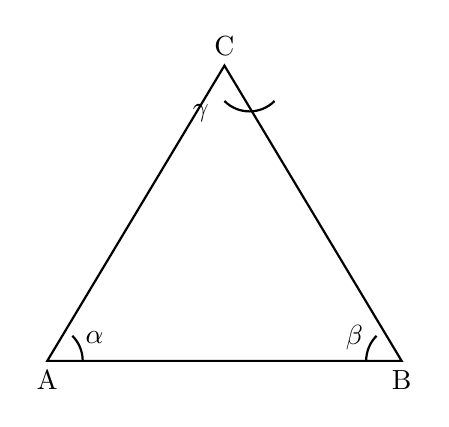
\begin{tikzpicture}[scale=1.5]
    \draw[thick] (0,0) -- (3,0) -- (1.5,2.5) -- cycle;
    \node[below] at (0,0) {A};
    \node[below] at (3,0) {B};
    \node[above] at (1.5,2.5) {C};
    
    % Angle marks
    \draw[thick] (0.3,0) arc (0:45:0.3);
    \node at (0.4,0.2) {$\alpha$};
    
    \draw[thick] (2.7,0) arc (180:135:0.3);
    \node at (2.6,0.2) {$\beta$};
    
    \draw[thick] (1.5,2.2) arc (225:315:0.3);
    \node at (1.3,2.1) {$\gamma$};
\end{tikzpicture}
\end{center}

\footnotesize
\texttt{\textbackslash draw[thick] (0.3,0) arc (0:45:0.3);}\\
\texttt{\textbackslash node at (0.4,0.2) \{\$\textbackslash alpha\$\};}
\end{frame}